\chapter{Implementation}
\label{sec:implementation}

This chapter describes the implementation of the kernels in \emph{C}
(\cref{sub:impl_c}) and the wrappers used to interface with them from
\emph{Julia} (\cref{sub:impl_julia}). Additionally, \cref{sec:reproducibility}
describes how the code and experiments are managed and how to reproduce the
results.

\section{Reproducibility}
\label{sec:reproducibility}

Before tackling the implementation of the kernels, it is important to discuss
how the code and its dependencies are managed to ensure reproducibility. This is
addressed in this section, where we describe the decisions taken to maximize
reproducibility.

One of the main problems in machine learning research (and research in general)
is the lack of reproducibility of the results. There are a lot of factors that
contribute to this, such as the lack of documentation, the lack of code
availability, the lack of standardization of the experimental setup, etc.
\cite{alstonBeginnerGuideConducting2021}. In this work, one of the main
objectives is to make the experimental setup as reproducible as possible.

\subsection{Dependency management}%
\label{sub:dependency_management}

\begin{wrapfigure}{r}{.40\textwidth}
    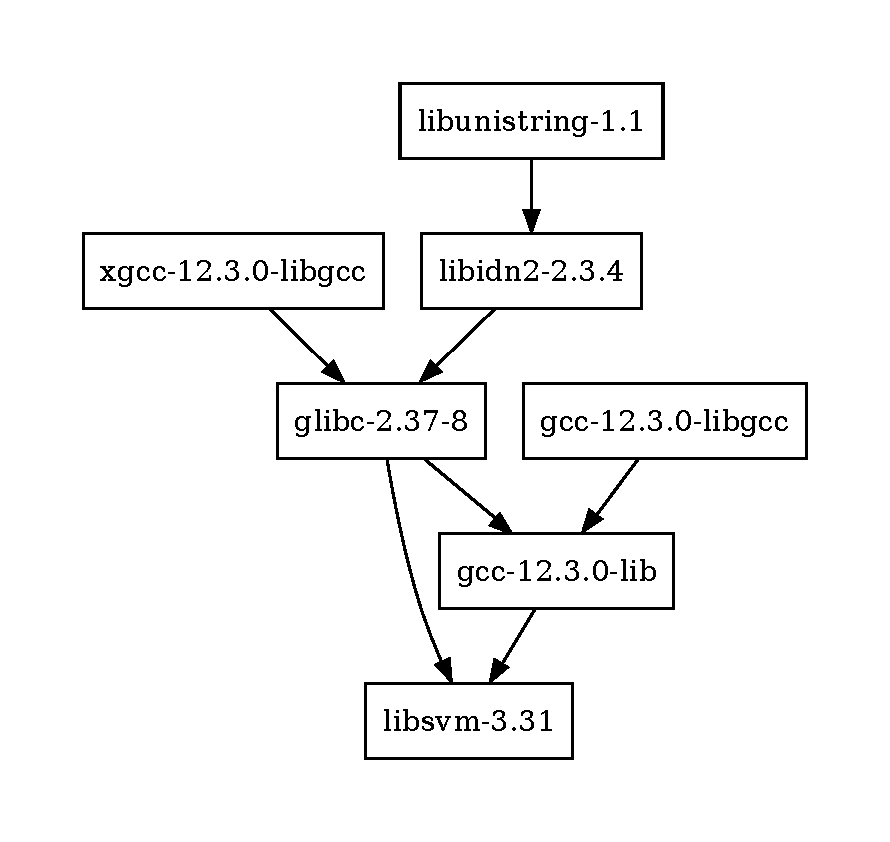
\includegraphics[width=.95\linewidth]{dependency_tree_libsvm}
    \caption{\libsvm runtime dependencies.}
    \label{fig:dependency_tree_libsvm}
\end{wrapfigure}

To manage the dependencies of the project, we use \emph{nix}
\cite{NixNixOSReproducible}, a purely functional package manager. \emph{Nix}
allows us to keep a consistent environment across different machines and
operating systems. It keeps track of \emph{all} the system dependencies of the
project including all the libraries and tools (such as compilers, interpreters,
etc.). For instance, with \emph{nix} we can visualize the runtime dependency
tree of the \libsvm library as shown in \cref{fig:dependency_tree_libsvm}.

On the \emph{Julia} side, the dependencies are managed through \emph{Pkg}
\cite{PkgJuliaLanguage}. All this complexity is hidden from the user through
\emph{direnv} \cite{DirenvUnclutterYoura}, which automatically loads the
environment when entering the project directory.

In summary, to reproduce the exact environment in which the experiments were
run, the user only needs to install \emph{nix} and \emph{direnv} and run
\texttt{direnv allow} in the project directory.

All the datasets used are publicly available and are downloaded automatically by
\emph{nix}. There is a file \texttt{datasets.toml} which contains the URLs of
the datasets and their checksums\footnote{The checksum uses
    \url{https://www.mankier.com/1/nix-hash}}, this guarantees that other users will
know if the dataset has been modified.

\begin{listing}[htpb]
    \caption{Fragment of the \texttt{datasets.toml} file.}
    \label{lst:datasets_toml}
    \inputminted[firstline=30,lastline=44]{toml}{../datasets.toml}
\end{listing}

\subsection{Build system}

To build the project, we use \emph{Nix} as well. The \emph{Nix} build system is
a declarative build system which allows us to specify the exact build steps and
dependencies of the project. Since the build steps are sandboxed with no access
to the system or the network, the build is guaranteed to be reproducible as long
as the process is deterministic (see \cref{sub:deterministic}).

\subsubsection{Determinism}
\label{sub:deterministic}

A deterministic build is a build that produces the same result given the same
inputs. There are many factors that can affect the result of a build, such as
the time of the build, the use of random numbers, race conditions, network
access, etc.

To mitigate these factors, where possible, we use a fixed seed for the random
number generator in \emph{Julia} and set the \texttt{SOURCE\_DATE\_EPOCH}
environment variable to a fixed date. The only factor that we do not control is
the execution order of different processes when running in parallel. However,
the multiple processes do not interact with each other in our case, so this
should not affect the result.

\subsection{Version control}

All versions of the code are stored in a \emph{git} repository hosted on GitHub.
% TODO: link to repo Additionally, all executions of experiments that generate
data, store the commit hash of the repository in which the code was run. This
allows us to trace back the exact version of the code used to generate the data.
This is handled through the \texttt{DrWatson.jl} package
\cite{datserisDrWatsonPerfectSidekick2020a}.

\subsection{Storing the results}

The \emph{DrWatson.jl} package also provides a mechanism to store the results of
the experiments, in which the results are serialized and stored in a \emph{JLD2}
file (a julia-specific version of the \emph{HDF5} format). Additionally, it
stores several metadata fields such as the commit hash, the parameters used and
other information such as the computed performance metric or any other relevant
information we may need. The filename for each result saved is generated from
the relevant parameters, which allows checking whether a certain parameter
configuration has already been computed and load it instead of recomputing it.

These \emph{JLD2} files contain the whole state of the trained machine models,
which is useful to be able to load the models and inspect them later. However,
this also means that the files are quite large (several hundred megabytes). For
most analysis we are only interested in the performance metric of the model, so
along with the \emph{JLD2} files, we also store a \emph{CSV} file with the
relevant information for each model. This allows us to quickly load the results
and perform analysis on them and, if necessary, we can load the full model from
the \emph{JLD2} file. This workflow is illustrated in
\cref{fig:experiment_flowchart}.

\begin{figure}[H]
    \begin{tikzpicture}
        % card with bullet points
        \node[draw, rectangle, minimum width=5cm, minimum height=3cm] (card) at (0,0) {};
        \node[anchor=north west] at (card.north west) {\textbf{Experiment\_1}};
        \node[anchor=north west] at ($(card.north west)+(0.2,-0.5)$) {- \texttt{sigma} = 0.1};
        \node[anchor=north west] at ($(card.north west)+(0.2,-1)$) {- \texttt{epsilon} = 0.5};
        \node[anchor=north west] at ($(card.north west)+(0.2,-1.5)$) {- \texttt{kernel} = \texttt{ArcSin}};
        \node[anchor=north west] at ($(card.north west)+(0.2,-2)$) {- \texttt{dataset} = \texttt{Triazines}};
        \node[anchor=north west] at ($(card.north west)+(0.4,-2.5)$) {\dots};

        \node (name) [below=of card] {\texttt{ex1\_sigma=0.1\_epsilon=0.5}\dots\texttt{.jld2}};
        \draw[-] (card) -- (name) node[midway, anchor=west] { filename};

        % if file exists, else

        \node[draw, diamond] (if) [below=of name] {Exists?};
        \draw[->] (name) -- (if);
        \node[draw, rectangle, rounded corners, inner sep = 10pt] (load) [left =of if] {Load};
        \node[draw, rectangle, rounded corners, inner sep = 10pt] (run) [right=of if] {Run};
        \draw[->] (if) -- (load) node[midway, anchor=south] {yes};
        \draw[->] (if) -- (run) node[midway, anchor=south ] {no};

        \coordinate [right=of name] (nameright) {};
        \node (csv) [right=of nameright] {\texttt{ex1\_results.csv}};

        \draw[-] (run.east) -| (nameright) node[midway, anchor=south west] {save};
        \draw[->] (nameright) |- (name);

        \draw[->] (run.east) -| (csv.south) node[midway, anchor=south west] {append};
    \end{tikzpicture}
    \caption{Flowchart of the experiment execution and results storage.}
    \label{fig:experiment_flowchart}
\end{figure}

\subsection{Running the experiments}

All the relevant code to the experiments is contained in the \texttt{src}
directory and scripts that run the experiments are in the \texttt{scripts}
directory and named after their corresponding experiment. To run an experiment,
we can simply call the corresponding \emph{Julia} script:
\mintinline{bash}{julia scripts/experiment_1.jl}. The dependencies can be
installed automatically using \emph{Nix} and \emph{direnv} as described in
\cref{sub:dependency_management}, with \mintinline{bash}{direnv allow} or
\mintinline{bash}{nix develop}.

Additionally, the \mintinline{bash}{nix build} command can be used to build the
document and a tarball with the datasets.

\section{Extending \libsvm{}}%
\label{sub:impl_c}

\libsvm is a C library developed by \textcite{CC01a} under BSD-3 license
which implements the Support Vector Machine (SVM) algorithm. The library is the
de facto standard for SVM implementations in the machine learning community,
being used by many other libraries and frameworks such as Python's
sklearn~\cite{ScikitlearnScikitlearn2023} or R's
e1071~\cite{meyer[autE1071MiscFunctions2023}.

Out of the box, \libsvm supports using the built-in kernels: linear,
polynomial, radial basis function (RBF) and sigmoid. Additionally, it can use
precomputed kernel matrices by setting the kernel type to \texttt{PRECOMPUTED}
and passing the kernel matrix as the training data.

The use of precomputed kernel matrices allows us to use any kernel function
of our choice. However, this requires computing the kernel matrix in advance,
which is not feasible for large datasets, since it requires $O(n^2)$ memory and
$O(n^2d)$ time, where $n$ is the number of samples and $d$ is the number of
features.
Instead, we can extend the library to add our own kernel functions
and let \libsvm compute the values as needed.
The \libsvm library is quite efficient in caching the kernel evaluations
and since it uses a Sequential Minimal Optimization algorithm, it only requires
some columns of the kernel matrix at a time \cite{CC01a}.

\subsection{Adding the kernels}

For our purposes, we want to extend the library by adding our own kernels. To do
so, we need to modify the library source by adding the corresponding kernel
functions. The kernel type is specified through an \texttt{enum}, so we can add
our own kernels to it and extend the switch statements in the code to handle
them. The modification is thus quite straightforward.
\cite{arquemartinezDissenyImplementacioEstudi2021}

From there, we have to implement the kernel functions themselves. Surprisingly
at first, the kernel functions are duplicated in the code for each kernel type:
\texttt{k\_function} and \texttt{kernel\_function}. The former is used for the
training phase and the latter for the prediction phase. This is explained in the
\libsvm{}'s FAQ \cite{LIBSVMFAQ}:

For the RBF kernel, Instead of doing $\exp\left(-\gamma\|x_i - x_j\|^2\right)$,
it computes $\exp\bigl(-\gamma(\|x_i\|^2 - 2x_i^Tx_j + \|x_j\|^2)\bigr)$, and by
precomputing $\|x_i\|^2$ for all $x_i$ in the beginning, the number of
operations is reduced from $3n$ to $2n$. This same optimization can be applied
to our kernels. \Cref{fig:c_improvement} shows the improvement in performance
when using this optimization (\emph{RadialBasis} is included as a check to make
sure it behaved the same in both cases, which it does).
The improvement is specially significant for the
normalized arc sine kernel since it requires more computations of the
dot product.

% \begin{cnote}
%     The plot probably should be improved:
%     Better legend, change labels and remove RBF since it is not relevant.
%     Also, add error bars?
% \end{cnote}
% TODO: Improve plot and explain better what is shown:
% - Better legend
% - Consistent colors with other kernel plots
% - probably make height smaller
\begin{figure}[H]
    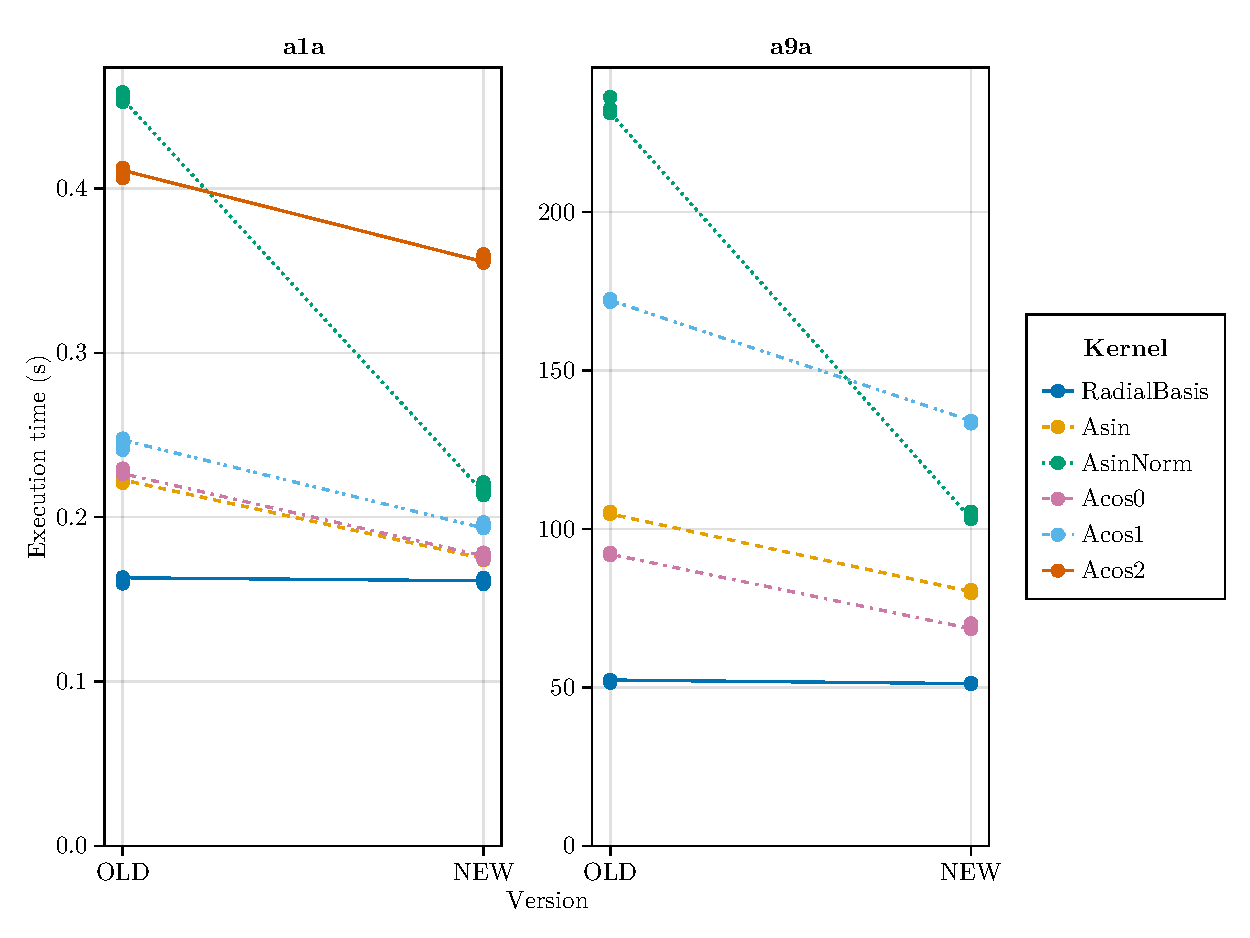
\includegraphics{plots/benchmark_time_improvement_old}
    \caption{Comparison between kernels on the training phase with and without
        pre-computation when training the Adult dataset}%
    \label{fig:c_improvement}
\end{figure}

The first step, is to add the new kernel types to the \texttt{enum} in
\texttt{svm.h} as shown in \cref{lst:svm_h_enum}.
\begin{listing}[H]
    \caption{Modified Enum definition from \texttt{svm.h}}
    \label{lst:svm_h_enum}
    \begin{minted}{C}
enum { LINEAR, POLY, RBF, SIGMOID, PRECOMPUTED, ASIN, ASIN_NORM, ACOS_0, ACOS_1, ACOS_2, ACOS_1_NORM, ACOS_2_NORM}; /* kernel_type */
\end{minted}
\end{listing}
Then, we add the corresponding cases to the switch statements in
\texttt{svm.cpp} for both \texttt{k\_function} and \texttt{kernel\_function} as
shown in \cref{lst:kernel_function}. The prediction case (\texttt{k\_function})
is not shown for brevity, but it is similar to the training case. The only
difference is the use of the precomputed dot product of $x_i$ with itself
(\texttt{x\_square}), which is passed as a parameter to the kernel function (See
\cref{lst:svm_cpp_k_function} in the appendix)

In order to avoid code duplication and make the code more readable, we added the
helper functions for the \texttt{asin} kernel shown in
\cref{lst:svm_cpp_helper}.

Another minor optimization for the \texttt{asin} kernel, instead of computing
$\frac{1}{2\sigma_w^2}$ every time as shown in the original
\cref{eq:kernel_asin}, we define $\gamma = \frac{1}{2\sigma_w^2}$ and pass it as
a parameter to the kernel function.

\begin{listing}[H]
    \caption{Helper functions for the asin kernel (\texttt{svm.cpp})}
    \label{lst:svm_cpp_helper}
    \begin{minted}{C}
// Passing x_square and y_square as parameters, we can avoid computing them again
// every time we call the kernel function
static inline double asin_elm(const svm_node *x, const svm_node *y, const double x_square, const double y_square, const double gamma) {
    return asin((1.0 + dot(x, y))/sqrt( (gamma + 1.0 + x_square)* (gamma + 1.0 + y_square)) );
};

// Alternative method used in prediction, where we don't have x_square and y_square precomputed
static inline double asin_elm(const svm_node *x, const svm_node *y, const double gamma) {
    return asin_elm(x, y, dot(x), dot(y), gamma);
}

// AsinELM with x=y, for faster computation, we don't need to compute the sqrt
static inline double asin_elm_equal(const double x_square, const double gamma) {
    const double x_square_plus_one = 1.0 + x_square;
    return asin(x_square_plus_one/(gamma + x_square_plus_one));
}
\end{minted}
\end{listing}

\begin{listing}
    \caption{Implementation of the kernels in \texttt{svm.cpp} for the training phase. \\[0.5em]
        (Notice the use of \texttt{x\_square} to avoid computing the dot product of $x$ with itself every time)
    }
    \label{lst:kernel_function}
    \begin{minted}[autogobble,mathescape,codetagify=NOTE]{C}
    double kernel_asin(int i, int j) const {
        return M_2_PI*asin_elm(x[i], x[j], x_square[i], x_square[j], gamma);
        // $\frac{2}{\pi}\arcsin\left(\frac{1 + x^Ty}{\sqrt{(1 + x^Tx)(1 + y^Ty)}}\right)$
    }
    double kernel_asin_norm(int i, int j) const {
        return asin_elm(x[i], x[j], x_square[i], x_square[j], gamma)/sqrt(
            asin_elm_equal(x_square[i], gamma)*asin_elm_equal(x_square[j], gamma)
        ); // NOTE: we use asin_elm_equal to avoid unnecessary sqrt computations
    }
    double kernel_acos_0(int i, int j) const {
        return 1.0 - M_1_PI*acos(dot(x[i], x[j])/sqrt(x_square[i]*x_square[j])); // $1 - \frac{\theta}{\pi}$
    }
    double kernel_acos_1(int i, int j) const {
        const double x2y2 = x_square[i]*x_square[j]; // $\lVert x \rVert^2 \lVert y \rVert^2$
        const double xy = sqrt(x2y2);                // $\lVert x \rVert \lVert y \rVert$
        const double cos_theta = dot(x[i], x[j])/xy; // $\cos(\theta) = \frac{x^Ty}{\lVert x \rVert \lVert y \rVert}$
        const double theta = acos(cos_theta);
        return M_1_PI*xy*(sin(theta) + (M_PI - theta)*cos_theta); // $\frac{1}{\pi}\lVert x \rVert \lVert y \rVert \left(\sin(\theta) + (\pi - \theta)\cos(\theta)\right)$
    }
    double kernel_acos_2(int i, int j) const {
        const double x2y2 = x_square[i]*x_square[j];         // $\lVert x \rVert^2 \lVert y \rVert^2$
        const double cos_theta = dot(x[i], x[j])/sqrt(x2y2); // $\cos(\theta) = \frac{x^Ty}{\lVert x \rVert \lVert y \rVert}$
        const double cos2_theta = cos_theta*cos_theta;
        const double theta = acos(cos_theta);
        return M_1_PI*x2y2*(3*sin(theta)*cos_theta + (M_PI - theta)*(1 + 2*cos2_theta)); // $\frac{1}{\pi}\lVert x \rVert^2 \lVert y \rVert^2 \left(3\sin(\theta)\cos(\theta) + (\pi - \theta)(1 + 2\cos^2(\theta))\right)$
    }
    double kernel_acos_1_norm(int i, int j) const {
        const double cos_theta = dot(x[i], x[j])/sqrt(x_square[i]*x_square[j]); // $\cos(\theta) = \frac{x^Ty}{\lVert x \rVert \lVert y \rVert}$
        const double theta = acos(cos_theta);
        return M_1_PI*(sin(theta) + (M_PI - theta)*cos_theta); // $\frac{1}{\pi}\left(\sin(\theta) + (\pi - \theta)\cos(\theta)\right)$
    }
    double kernel_acos_2_norm(int i, int j) const {
        const double cos_theta = dot(x[i], x[j])/sqrt(x_square[i]*x_square[j]); // $\cos(\theta) = \frac{x^Ty}{\lVert x \rVert \lVert y \rVert}$
        const double cos2_theta = cos_theta*cos_theta;
        const double theta = acos(cos_theta);
        return M_1_PI*(3*sin(theta)*cos_theta + (M_PI - theta)*(1 + 2*cos2_theta)); // $\frac{1}{\pi}\left(3\sin(\theta)\cos(\theta) + (\pi - \theta)(1 + 2\cos^2(\theta))\right)$
    }
\end{minted}
\end{listing}

\subsubsection{A Note on the possibility of passing the kernel as a function pointer}

One of the initial ideas was to pass the kernel function as a parameter to the
library. This would mean that the kernel function would be implemented in
\emph{Julia} and passed to the library as a function pointer. However, this
requires extensive modification of the library and a high performance
penalty. This is because the kernel function is called many times and the
\libsvm kernels are constant functions that are inlined by the
compiler. Passing the kernel as a function pointer introduces both a function
call and a pointer dereference, which is a significant performance penalty. For
these reasons, we decided to implement the kernels directly in the library.

\subsection{Controlling the number of iterations}

A Support Vector Machine (SVM) is a quadratic optimization problem, which
in \libsvm is solved using the Sequential Minimal Optimization (SMO).
The SMO algorithm is an iterative algorithm which stops when the KKT conditions
are satisfied. The number of iterations the algorithm takes depends on both
the dataset and the parameters. A bad choice of parameters can lead to a very
slow convergence \cite{CC01a}.

One metric which we wanted to measure was the number of iterations the SMO
algorithm took and have the possibility to stop it early.
\libsvm only provides a \texttt{tolerance} parameter for the stopping
criterion. However, in \emph{sklearn} they provide a \texttt{max\_iter}
parameter\footnote{\url{https://github.com/scikit-learn/scikit-learn/pull/1184}}
which is the maximum number of iterations and also report the number of
iterations the algorithm took
\footnote{\url{https://github.com/scikit-learn/scikit-learn/pull/21408}}. This
is accomplished by using a modified version of \libsvm{}. Since we are
modifying the library as well, we added the same functionality to our modified
version. This is something were the \emph{Julia} wrapper of \libsvm is
lacking when compared to the more mature \emph{Python} version.

\pagebreak % INFO: make sure this is start of page so wrapfigure plays nice
\section{Julia}%
\label{sub:impl_julia}

\begin{wrapfigure}{r}{.40\textwidth}
    
\includegraphics[width=.95\linewidth]{julia-logo-color}
    \caption{Julia logo.\protect\footnotemark}
    \label{fig:julia_logo}
\end{wrapfigure}
\footnotetext{Official Julia logo by Stefan Karpinski, licensed under \href{https://creativecommons.org/licenses/by-sa/4.0/}{CC BY-SA 4.0}.}

\emph{Julia} \cite{bezanson2017julia} is a high-level, high-performance dynamic
programming language which is designed from the ground up to be fast,
expressive, and easy to write. Its aim is to provide the ease of use of a
scripting language such as Python while being as fast as a compiled language
such as C. In particular, \emph{BinaryBuilder.jl}
\cite{JLLPackagesBinaryBuilder} allows reproducible cross-platform compilation
of 3rd party libraries for different platforms and architectures. This is used
throughout the Julia ecosystem to provide binary dependencies for packages, for
example, \libsvm is provided by the \emph{libsvm\_jll} package
\cite{LibsvmJllJl2022}. This makes it very easy to modify the \libsvm
library used by a package by simply updating the dependency to our modified
\emph{libsvm\_jll} package.

The latest stable version at the time of writing (1.9.x) introduced a major
improvement on the time to first execution, which historically has been one of
the main drawbacks of the language. In previous versions, every new session had
to pre-compile all the libraries as they were loaded, which often could take
minutes. Now, this is cached between sessions\cite{JuliaV1Release}.

For the above reasons, along with the fact that there is a large and growing
number of machine learning packages in Julia, we decided to interface our
modified \libsvm library with Julia.

\subsection{libsvm\_jll}

As mentioned before, the \emph{libsvm\_jll} package is a compiled version of the
\libsvm C library compiled through \emph{BinaryBuilder.jl}. This so-called
\emph{Julia Link Library} (JLL) package is not much different from a regular
system library, except that its dependencies are dynamically linked to other JLL
packages.

For our implementation, we used the original recipe from
\textcite{LibsvmJllJl2022} and modified it to use our modified \libsvm
source code.

\subsection{LIBSVM.jl}

The \emph{LIBSVM.jl} package \cite{LIBSVMJl2023} is a Julia wrapper that
provides a high-level interface to the \libsvm library. It uses the artifacts
generated by the \emph{libsvm\_jll} package and provides the
translation between Julia types and the C types.

\subsubsection{Adding the kernels}

The kernels can be added by extending the \texttt{Kernel} \texttt{enum} in Julia
to reflect the \texttt{enum} in the C library.
\begin{listing}[H]
    \begin{minted}{julia}
module kernel
@enum KERNEL Linear Polynomial RadialBasis Sigmoid Precomputed Asin AsinNorm Acos0 Acos1 Acos2 Acos1Norm Acos2Norm
end
\end{minted}
    \caption{Julia \texttt{enum} definition for the kernels, equivalent to the C definition in \cref{lst:svm_h_enum}.}
    \label{lst:kernel_enum_julia}
\end{listing}

Technically, this is the only change needed to add the kernels to the library,
since the \emph{C} library has the kernel functions implemented and selects them
based on the kernel type enum.

\subsubsection{Adding the number of iterations}

The modification of the number of iterations is a little more involved and
requires modifying the \texttt{SVMModel} and \texttt{SVMParameter} types to
store the number of iterations as well as properly copying the values from the C
pointer into Julia object. In order to test that this was properly implemented,
we added a test set to \emph{LIBSVM.jl}. The tests validate that the number of
iterations copied from the C pointer is the same as the one returned by the
\libsvm library and that \texttt{max\_iter} is respected.

\subsubsection{\libsvm 3.31}

The version of \libsvm used by \emph{LIBSVM.jl} is 3.25. It has not been
updated to the newest version 3.31, since it breaks the API by adding the option
of probability density estimation. Again, we worked around this by modifying the
library to properly handle the new API (this change will be upstreamed to
\emph{LIBSVM.jl}). % TODO: link to PR

\subsection{MLJ}

\emph{MLJ} \cite{blaomMLJJuliaPackage2020} is a machine learning framework for
Julia which provides a common interface for many machine learning packages. It
is the equivalent of \emph{scikit-learn} in Python. It provides an interface to
\emph{LIBSVM.jl} through the \emph{MLJLIBSVMInterface.jl} package. By modifying
the latter package to include the \texttt{max\_iter} parameter, we can use it in
\emph{MLJ}.

From this point, we can use all the functionality provided by \emph{MLJ} to
train, evaluate, tune and visualize our SVM models with flexibility and ease.

\Cref{fig:julia_libsvm_deps} shows the relationship between the packages and how
the libraries interface with each other.

\begin{figure}[H]
    \begin{tikzpicture}[
            box/.style={draw, rectangle, minimum width=1cm, minimum height=1cm},
            C/.style={fill=wong_blue!40,postaction={pattern=north west lines,pattern color=wong_blue!10}},
            Julia/.style={fill=wong_green!70},
            JLL/.style={fill=wong_orange!70,postaction={pattern=north east lines,pattern color=wong_orange!10}},
        ]
        \node[box,C] (libsvm) at (0,0) {libsvm};
        \node[box,JLL,below=of libsvm] (libsvm_jll) {libsvm\_jll};
        \node[box,Julia,right=of libsvm_jll] (LIBSVM) {LIBSVM.jl};
        \node[box,Julia,right=of LIBSVM] (MLJLIBSVMInterface) {MLJLIBSVMInterface.jl};
        \node[box,Julia,below=of MLJLIBSVMInterface] (MLJ) {MLJ.jl};

        \draw[->] (libsvm) -- (libsvm_jll) node[midway, anchor=west,color=wong_green] {build\_tarballs.jl};
        \draw[->] (libsvm_jll) -- (LIBSVM);
        \draw[->] (LIBSVM) -- (MLJLIBSVMInterface);
        \draw[->] (MLJLIBSVMInterface) -- (MLJ);

        % Color Legend
        \matrix [draw,right] at ($(current bounding box.east)+(0.5,0)$) {
            \node [C,label=right:C] {};                    \\
            \node [JLL,label=right:Julia Link Library] {}; \\
            \node [Julia,label=right:Julia] {};            \\
        };

    \end{tikzpicture}
    \caption{Dependency graph of Julia packages exposing the \libsvm library API.}
    \label{fig:julia_libsvm_deps}
\end{figure}

The forked versions of the libraries discussed in this section can be found in
the following repositories:
\begin{itemize}
    \item \url{https://github.com/LeixB/libsvm}
    \item \url{https://github.com/Leixb/build\_tarballs\_libsvm\_jll}
    \item \url{https://github.com/Leixb/libsvm\_jll.jl}
    \item \url{https://github.com/LeixB/LIBSVM.jl}
    \item \url{https://github.com/LeixB/MLJLIBSVMInterface.jl}
\end{itemize}

% \subsection{Memoization}
% TODO: Check if memoization if worth it or if we can do it manually in a more
% sensible way.

\subsection{Visualizing the kernels}

Once all the kernels are implemented and the \emph{Julia} interface through
\emph{MLJ} is also complete, we can try to run the kernels to produce some
plots and compare them with the equivalent plots from the literature.

\begin{figure}[H]
    \begin{subfigure}{.59\textwidth}
        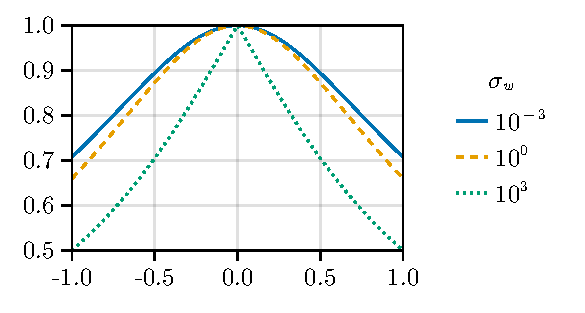
\includegraphics{plots/kernel_asin}
        \caption{Our custom implementation}
    \end{subfigure} \begin{subfigure}{.40\textwidth}
        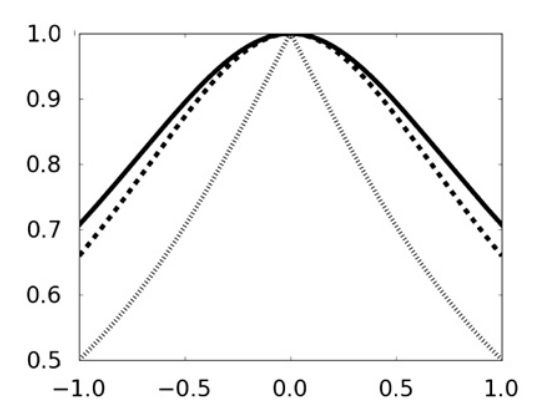
\includegraphics{frenay-kernel}
        \caption{\textcite{frenayParameterinsensitiveKernelExtreme2011}}
    \end{subfigure}
    \caption{Normalized Asymptotic ELM kernel evaluated around 0}
    \label{fig:kernel_asin_comparison}
\end{figure}

\Cref{fig:kernel_asin_comparison} shows the result of plotting the normalized
asymptotic ELM kernel around 0 through our implementation in \emph{Julia} and
the equivalent plot given in the original paper (the legend applies to both
plots).

\begin{cnote}
    Arc cosine kernels cannot be easily visualized in 2d, since 0 is undefined.
    Also, they look like their activation functions when plotted as done
    with asin.
\end{cnote}

% TODO: maybe add this?
% \subsection{Passing the kernel as a function pointer}
%
% One of the ideas explored was to instead of hard-coding the kernels in the
% library, set the kernel as a function pointer in libsvm. This would allow
% to define a function in Julia, get it's pointer and pass it to libsvm. This
% approach was evaluated and discarded since it would require a major
% refactor of the libsvm library and the divergence from the original library
% would make further updates more difficult.
%
% It is technically possible and worth exploring in the future, but the
% architecture of the libsvm library is quite constricted.


\section{Meta learning}
\label{sec:meta-learning}

The trial and error approach of machine learning tasks is often tedious and
time-consuming. Driven by this, multiple approaches have been proposed to make
recommender systems, which take the results of simple experiments and metrics
(meta-features) and use them to recommend hyperparameter values, search spaces
and optimization algorithms for similar tasks. This process of using
meta-features is a form of meta-learning. \Textcite{rivolliMetafeaturesMetalearning2022}
provides a comprehensive survey of the different meta-features and meta-learning
approaches.

\begin{important}
    Add table with meta-features (probably in appendix? There are 60+)
\end{important}
\begin{description}
    % TODO: probably rewrite all this descriptions
    % TODO: table with all the used meta-features? There are ~60
    \item[General]: also referred to as simple, are features that can be
    extracted from the data easily, with little computational cost. In this
    category, we have the number of instances, number of attributes, number
    of numeric attributes, the ratio of instances to attributes, etc.

    \item[Statistical]: as the name implies, they capture statistical properties
    of the data: mean, standard deviation, skewness, kurtosis, etc.
    These are only applicable to numeric attributes.

    \item[Information theory]: based on entropy measures, they capture the
    complexity and amount of information in the data.
    Only applicable to categorical attributes.

    \item[Model-based]: extracted from measures on models trained on the data.
    Usually from decision trees. These include the number of leaves, the
    number of nodes, the maximum depth, etc.

    \item[Landmarking]: not to be confused with the model-based, these focus
    on the performance of simple models on the data.
\end{description}

Implementing the meta-features and meta-learning algorithms is out of the scope
of this work, so we will use the \emph{PyMFE} python
package~\cite{WelcomePyMFEDocumentation,JMLR:v21:19-348} which provides
a vast collection of the most common meta-features.

Julia provides a convenient way to call Python code and libraries through the
\emph{PyCall.jl} package, which allows us to use \emph{PyMFE} from Julia, an
example of this is shown in \cref{lst:metafeatures}.

\begin{listing}
    \caption{Using \emph{PyMFE} from Julia to extract meta-features from a datasets.}%
    \label{lst:metafeatures}
    \begin{minted}{julia}
module MetaFeatures

import ..DataSets: DataSet, unpack
using PyCall, DataFrames, ProgressMeter

export extract_features

const MFE = pyimport("pymfe.mfe").MFE

"Return a Dict with the meta-features extracted from the dataset using the pymfe library."
function extract_features(X, y, args...; features=MFE.valid_metafeatures(), kwargs...)
    mfe = MFE(args...; features, kwargs...)
    mfe.fit(Matrix(X), y, precomp_groups=["general", "model-based", "landmarking"])
    ft = mfe.extract()

    # Convert list of tuples [(a, 7), (b, 4), ...] to Dict {a => 7, b => 4, ...}
    zip(ft...) |> Dict
end

function extract_features(datasets::Vector{<:DataSet}, args...; kwargs...)
    features = @showprogress map(datasets) do ds
        @info "Extracting features from $(ds)"
        X, y = unpack(ds)
        ft = extract_features(X, y, args...; kwargs...) |> DataFrame
        ft.dataset = [string(ds)]

        ft
    end

    vcat(features..., cols=:union)
end

end # module MetaFeatures
    \end{minted}
\end{listing}


% TODO: statistical meta-features we don't use since they take too long
